\chapter{Espacios Recubridores}

\begin{observacion}
    A lo largo de este tema supondremos que todos los espacios topológicos son conexos y localmente arcoconexos. En particular estos espacios son siempre arcoconexos.
\end{observacion}

\section{Levantamiento de aplicaciones}

\begin{observacion}
    Vamos a tener en cuenta que si $X$ es un espacio topológico conexo y localmente arcoconexo, entonces todo abierto suyo cumple que cada componente arcoconexa es abierta.

    \begin{proof}
        Si $O$ es abierto y $A$ es una componente arcoconexa de $O$, entonces dado $a\in A$, como $X$ es localmente arcoconexo tendremos que existe un $U$ entorno arcoconexo de $a$ tal que $U\subseteq O$. Como $A$ es el mayor arcoconexo en $O$ que contiene al punto $a$ tendremos que $U\subseteq A$, luego $A$ es abierto.
    \end{proof}
    
    Esto lo vamos a usar para el caso en el que tenemos dada una aplicación recubridora $p:R\to B$ y un punto $b_0\in B$. Entonces tendremos que existe un abierto regularmente recubierto $O$ que contiene a $b_0$. Restringiéndonos a la componente arcoconexa de $O$ que contiene a $b_0$ podremos suponer que el entorno regularmente recubierto es abierto y arcoconexo.
\end{observacion}

\begin{lema}[Unicidad del levantamiento]
    Sean $p:R \to B$ una aplicación recubridora, $f_1,f_2:X\to R$ continuas tales que 
    \begin{gather*}
        p\circ f_1 = p\circ f_2
    \end{gather*}
    Si existe un $x_0\in X$ tal que $f_1(x_0)=f_2(x_0)$, entonces $f_1=f_2$.

    \begin{proof}
        Para la demostración solo se necesita que $X$ sea conexo y no necesariamente localmente arcoconexo. \\

        Partimos la siguiente situación
        \begin{gather*}
            \xymatrix{
                && R \ar[d]^{p}\\
                X \ar[urr]^{f_1,f_2} \ar[rr]_{f=p\circ f_1 = p\circ f_2} && B
            }
        \end{gather*}
        Consideramos el siguiente conjunto
        \begin{gather*}
            Y=\{x\in X : f_1(x)=f_2(X)\}
        \end{gather*}
        Como $X$ es conexo y tenemos que $Y \neq \emptyset$, ya que por hipótesis $x_0\in Y$, si probamos que $Y$ es abierto y cerrado tendremos que $Y=X$, es decir, $f_1=f_2$. \\
        
        Veamos que $Y$ es abierto. Para ello tomamos $y\in Y$, es decir, un punto $y$ tal que $f_1(y)=f_2(y)$. Elegimos el punto $b=p(f_1(y))=p(f_2(y))$. Sea $O$ abierto regularmente recubierto y arcoconexo que contiene a $b$, entonces 
        \begin{gather*}
            p^{-1}(O) = \bigcup\limits_{i\in I} A_i
        \end{gather*}
        donde los $A_i$ son abiertos disjuntos de $R$ y tal que 
        \begin{gather*}
            p_{|A_i}: A_i \to O
        \end{gather*} 
        es un homeomorfismo. Tomamos el abierto $A_{i_0}$ donde se encuentra $f_1(y)=f_2(y)$. Elegimos $V=f_1^{-1}(A_{i_0}) \cap f_2^{-1}(A_{i_0})$. Veamos que $\forall x \in V$ se tiene que $f_1(x)=f_2(x)$. Como $x\in V$ tendremos que $f_1(x),f_2(x)\in A_{i_0}$ por lo que 
        \begin{gather*}
            p(f_1(x)) = p(f_2(x)) \overset{(\ast)}{\Rightarrow} f_1(x)=f_2(x) \Rightarrow V\subseteq Y
        \end{gather*}
        donde en $(\ast)$ hemos usado que $p_{|A_i}$ es inyectiva. Tenemos finalmente que $Y$ es abierto.\\

        Veamos ahora que $Y$ es cerrado. Para ello demostramos que $X\setminus Y$ es abierto. Tomamos $y\in X\setminus Y$ y vemos que existe un $V$ abierto que contiene al punto $y$ y tal que $V\subseteq X \setminus Y$. Sea $b=p(f_1(y))=p(f_2(y))$ y de nuevo tomamos $O$ regularmente recubierto que contiene a $b$. Tendremos
        \begin{gather*}
            p^{-1}(O) = \bigcap\limits_{i\in I} A_i
        \end{gather*}
        donde los $A_i$ son abiertos disjuntos y tal que 
        \begin{gather*}
            p_{|A_i}: A_i\to O 
        \end{gather*}
        es un homeomorfismo. Tendremos $f_1(y)\in A_{i_1}$ y $f_2\in A_{i_2}$ y además se verificará que $A_{i_1}\neq A_{i_2}$ ya que si se diera la igualdad tendríamos que la aplicación
        \begin{gather*}
            p_{|A_{i_1}}: A_{i_1} \to O
        \end{gather*}
        no sería intectiva. Elegimos ahora $V=f_1^{-1}(A_1) \cap f_2^{-1}(A_2)$, donde se tiene que $y\in V$. Además se tiene que 
        \begin{gather*}
            f_1(V)\subseteq A_{i_1}\\
            f_2(V)\subseteq A_{i_2}
        \end{gather*}
        por lo que para cada $x\in V$ se tendrá que $f_1(x)\neq f_2(x)$ ya que $f_1(x)\in A_{i_1}$ y $f_2(x)\in A_{i_2}$. Esto nos dice que $V\subseteq X\setminus Y$, luego $Y$ es cerrado.
    \end{proof}
\end{lema}

\begin{teo}[Teorema de monodromía]
    Sean $p:R \to B$ una aplicación recubridora, $b_0\in V$ y $r_0\in p^{-1}(b_0)$. El homomorfismo inducido $p_*:\pi_1(R,r_0)\to \pi_1(B,b_0)$ es inyectivo. En partircular, $\pi_1(R,r_0)$ es isomorfo a $p_*(\pi_1(R,r_0))< \pi_1(B,b_0)$.

    \begin{proof}
        Sabemos que $p_*$ es inyectiva si y solo si $\ker(p_*)$ es trivial. Tomamos $\alpha$ lazo basado en $r_0$ tal que 
        \begin{gather*}
            p_*([\alpha]) = [\veps_{b_0}]
        \end{gather*}
        Como además $[p\circ \alpha] = p^*([\alpha])$ tenemos que existe una homotopía por lazos de $\veps_{b_0}$ en $p\circ \alpha$. Como toda homotopía por arcos se puede levantar tenemos que existe una homotopía por arcos en $R$ de $\hat{\veps}_{b_0}$ y $\widehat{p\circ \alpha}$ (empezando en $r_0$). Tenemos
        \begin{gather*}
            \left.
            \begin{array}{l}
                \hat{\veps}_{b_0} = \veps_{r_0}\\\\
                \widehat{p\circ \alpha} = \alpha
            \end{array}
            \right\}  \Rightarrow [\alpha] = [\veps_{r_0}]
        \end{gather*}
    \end{proof}
\end{teo}

\begin{observacion}
    Recordemos que dados dos subgrupos $H_1,H_2$ de un grupo $G$ se dice que $H_1$ y $H_2$ son conjugados si existe un $g\in G$ tal que 
    \begin{gather*}
        H_2=g^{-1}H_1 g
    \end{gather*}
\end{observacion}

\begin{coro}
    Sean $p:R \to B$ una aplicación recubridora, $b_0\in B$ y $r_1,r_2\in p^{-1}(b_0)$. Elegimos un arco $\alpha:[0,1]\to R$ tal que
    \begin{gather*}
        \alpha(0)=r_1\\
        \alpha(1)=r_2
    \end{gather*}
    entonces 
    \begin{gather*}
        p_*(\pi_1(R,r_2)) = [p\circ\alpha]^{-1} \ast p_*(\pi_1(R,r_1)) \ast [p\circ\alpha]
    \end{gather*}
    En particular, $p_*(\pi_1(R,r_1))$ y $p_*(\pi_1(R,r_2))$ son conjugados en $\pi_1(B,b_0)$.

    \begin{proof}
        Sabemos que $p\circ \alpha$ es un lazo basado en $b_0$ por lo que $[p\circ \alpha]\in \pi_1(B,b_0)$. Además,
        \begin{align*}
            \pi_1(R,r_2) &\overset{isom.}{\to} \pi_1(R,r_1)\\
            [\beta] &\mapsto [\alpha \ast \beta \ast \tilde{\alpha}]
        \end{align*}
        Tenemos por tanto que 
        \begin{gather*}
            \pi_1(R,r_1) = [\alpha] \ast \pi_1(R,r_2) \ast [\tilde{\alpha}]\\
            p_*(\pi_1(R,r_1)) = [p\circ \alpha] \ast p_*(\pi_1(R,r_2)) \ast [p\circ \tilde{\alpha}]
        \end{gather*}
        Como tenemos que 
        \begin{gather*}
            [p\circ \tilde{\alpha}] = [\tilde{p\circ \alpha}] = [p\circ \alpha]^{-1}
        \end{gather*}
        llegamos a que son conjugados.
    \end{proof}
\end{coro}

\begin{coro}
    Sean $p:R\to B$ una aplicación recubridora, $b_0\in B$ y $r_1\in p^{-1}(b_0)$. Sea $H$ un subgrupo conjugado de $p_*(\pi_1(R,r_1))$ en $\pi_1(B,b_0)$. Entonces existe un punto $r_2\in R$ tal que
    \begin{gather*}
        H=p_*(\pi_1(R,r_2))
    \end{gather*}
    \begin{proof}
        Por hipótesis sabemos que $p(r_1)=b_0$ y que $p_*(\pi_1(R,r_1))$ es conjugado con $H$ en $\pi_1(B,b_0)$, es decir, 
        \begin{gather*}
            H = g^{-1} \ast p_*(\pi_1(R,r_1)) \ast g
        \end{gather*}
        con $g\in \pi_1(B,b_0)$, esto es, $g=[\gamma]$. Consideramos $\hat{\gamma}$ el levantamiento de $\gamma$ a $R$ con 
        \begin{gather*}
            \hat{\gamma}(0) = r_1
        \end{gather*}
        y llamamos $r_2=\hat{\gamma}(1)$ al final del arco.
        \begin{gather*}
            p(r_2) = (p\circ \hat{\gamma})(1) = \gamma(1) = b_0
        \end{gather*}
        Usando el corolario anterior tenemos que 
        \begin{align*}
            p_*(\pi_1(R,r_2)) &= [p\circ \hat{\gamma}]^{-1} \ast p_*(\pi_1(R,r_1)) \ast [p\circ \hat{\gamma}] =\\
            &= [\gamma]^{-1} \ast p_*(\pi_1(R,r_1)) \ast [\gamma] =\\
            &= H
        \end{align*}
    \end{proof}
\end{coro}

\begin{teo}
    Consideramos una aplicación recubridora $p:R\to B$, una aplicación continua $f:X\to B$, $x_0\in X$, $b_0=f(x_0)$ y $r_0\in p^{-1}(b_0)$. 
    
    \begin{gather*}
        \xymatrix{
            & R \ar[d]^p\\
            X \ar[r]^{f} \ar@{-->}[ur]^{\hat{f}} & B
        }
    \end{gather*}

    Entonces son equivalentes:
    \begin{enumerate}
        \item Existe un levantamiento $\hat{f}:X \to R$ de $f$ con $\hat{f}(x_0)=r_0$.
        \item $f_*(\pi_1(X,x_0))\subseteq p_*(\pi_1(R,r_0))$
    \end{enumerate}
    Además, si se cumple cualquiera de estas condiciones, el levantamiento $\hat{f}$ de $f$ con $\hat{f}(x_0)=r_0$ es único.

    \begin{proof}\
        \begin{itemize}
            \item [(1) $\Rightarrow$ (2)] Estamos en la situación del siguiente diagrama
            \begin{gather*}
                \xymatrix{
                    & \pi_1(R,r_0) \ar[d]^{p_*}\\
                    \pi_1(X,x_0) \ar[ur]^{\hat{f}_x} \ar[r]_{f_*} & \pi_1(B,b_0)
                }
            \end{gather*}
            y podemos ver que 
            \begin{gather*}
                f_*(\pi_1(X,x_0)) = p_*(\hat{f}_*(\pi_1(X,x_0))) \subseteq p_*(\pi_1(R,r_0))
            \end{gather*}
            ya que $\hat{f}_*(\pi_1(X,x_0))\subseteq \pi_1(R,r_0)$ por lo que tenemos esta implicación simplemente desarrollando la composición.

            \item [(2) $\Rightarrow$ (1)] Empezamos definiendo $\hat{f}$:
            \begin{gather*}
                \xymatrix{
                    & R \ar[d]^p\\
                    X \ar[r]^f & B
                }
            \end{gather*}
            Dado $x\in X$ elegimos $\alpha_x$ un arco en $X$ que una $x_0$ con $x$. Entonces $f\circ \alpha_x$ es un arco en $B$ que une $b_0 = f(x_0)$ con $f(x)$. Consideramos ahora $\widehat{f\circ \alpha_x}$ el único arco en $R$ tal que $\widehat{f\circ \alpha_x}(0) = r_0$ y definimos 
            \begin{gather*}
                \hat{f}(x) = \widehat{f\circ \alpha_x}(1)
            \end{gather*}
            Veamos que $\hat{f}$ está bien definida, es decir, que no depende del arco $\alpha_x$ elegido. Tomamos otro arco $\beta_x$ en $X$ tal que $\beta_x(0)=x_0$ y $\beta_x(1)=x$ y queremos ver que
            \begin{gather*}
                \widehat{f\circ \alpha_x}(1) = \widehat{f\circ \beta_x}(1)
            \end{gather*}

            Tomamos $\gamma=\alpha_x \ast \tilde{\beta_x}$ que es un lazo en $X$ con base en $x_0$. Tenemos entonces que 
            \begin{gather*}
                f \circ \gamma = (f\circ \alpha_x) \ast (f \circ \tilde{\beta_x})
            \end{gather*}
            es un lazo con base en $b_0$. Usamos ahora la hipótesis y tenemos que 
            \begin{gather*}
                [f\circ \gamma] = f_*([\gamma]) \in p_*(\pi_1(R, r_0))
            \end{gather*}
            Es decir, existe un arco $\delta$ con base en $r_0$ tal que $[f\circ \gamma] = [p\circ \delta]$. Sea $\widehat{f\circ \gamma}$ el único levantamiento de $f\circ \gamma$ que comienza en $r_0$. Tenemos que $f\circ \gamma$ es homotópico por arcos con $p\circ \delta$. Como $p_*$ es inyectiva tenemos que $\widehat{f\circ \gamma}$ es homotópico con $\delta$, por lo que ambos acaban en el mismo punto, es decir, tenemos que 
            \begin{gather*}
                \widehat{f\circ \gamma}(1) = \delta(1) = r_0
            \end{gather*}
            Además tenemos que 
            \begin{gather*}
                \widehat{f\circ \gamma} = \widehat{(f\circ \alpha_x) \ast \tilde{f\circ \beta_x}} = \widehat{f\circ \alpha_x} \ast \omega
            \end{gather*}
            donde $\widehat{f \circ \alpha_x}$ es el levantamiento de $f\circ \alpha_x$ empezando en $r_0$ y $\omega$ es el levantamiento de $\tilde{f\circ \beta_x}$ comenzando en $\widehat{f\circ \alpha_x}(1)$. Podemos ver que 
            \begin{gather*}
                 \left.
                \begin{array}{c}
                    p\circ \omega = \tilde{f\circ \beta_x} = f\circ \tilde{\beta_X}\\
                    \omega(1) = r_0\\
                    \omega(0) = \widehat{f\circ \alpha_x}(1)
                \end{array}
                \right\} \Rightarrow
                \begin{array}{c}
                    p\circ \tilde{\omega} = f\circ \beta_x\\
                    \tilde{\omega}(0) = \omega(1) = r_0\\
                    \tilde{\omega}(1) = \omega(0) = \widehat{f\circ \alpha_x}(1)
                \end{array}
            \end{gather*}
            Por tanto
            \begin{gather*}
                \widehat{f\circ \beta_x}(1) = \tilde{\omega}(1)=\widehat{f\circ \alpha_x}(1)
            \end{gather*}
            lo que demuestra que la definición de $\hat{f}(x)$ está bien hecha.\\

            Veamos ahora que $p\circ \hat{f}=f$. Para ello, dado $x\in X$ tenemos que ver que $(p\circ \hat{f})(x) = f(x)$. Veamos quién es $\hat{f}(x)$:
            \begin{gather*}
                \hat{f}(x) = \widehat{f\circ \alpha_x}(1)\\
                p(\hat{f}(x)) = (p\circ (\widehat{f\circ \alpha_x}))(1) = (f\circ \alpha_x)(1) = f(\alpha_x(1)) = f(x)
            \end{gather*}
            También es claro que $\hat{f}(x_0)=r_0$ ya que para $x_0$ podemos elegir $\veps_{x_0}$ verificándose que $f\circ \veps_{x_0} = \veps_{b_0}$ luego 
            \begin{gather*}
                \widehat{f\circ \veps_{x_0}} = \hat{\veps}_{b_0} = \veps_{r_0} \Rightarrow \hat{f}(x_0) = \widehat{f\circ \veps_{x_0}}(1) = \veps_{r_0}(1) = r_0
            \end{gather*}
            Vamos a demostrar ahora que $\hat{f}$ es continua. 
            \begin{gather*}
                \xymatrix{
                    & R \ar[d]^p\\
                    X \ar[ur]^{\hat{f}} \ar[r]^f & B
                }
            \end{gather*}
            Comenzamos tomando un punto $x\in X$ y vemos que $\hat{f}$ es continua en $x$. Sea $U$ un entorno de $\hat{f}(x)$. Tomamos $O$ abierto arcoconexo de $f(x)$ que esté regularmente recubierto, es decir
            \begin{gather*}
                p^{-1}(O) = \bigcup\limits_{i\in I} A_i \text{ con } A_i \text{ disjuntos}\\
                p_{|A_i} : A_i \to O \text{ homeomorfismo}
            \end{gather*}
            Como $\hat{f}(x)\in p^{-1}(f(x))\subseteq p^{-1}(O)$ tenemos que existe un único $i_0\in I$ tal que $\hat{f}(x)\in A_{i_0}$. Podemos suponer que $A_{i_0}\subseteq U$ (si no fuese así consideraríamos $U\cap A_{i_0}$). Como $f$ es continua, existe un abierto $V$ que contiene a $x$ tal que $f(V)\subseteq O$. Podemos suponer que $V$ es arcoconexo (si no lo fuese podríamos coger la componente arcoconexa de $V$ que contenga a $x$).\\
            
            Si probamos que $\hat{f}(V)\subseteq A_{i_0}\subseteq U$ tendríamos que $\hat{f}$ es continua en $x$. Para verlo consideramos un punto $y\in V$ y tomamos un arco $\gamma$ dentro de $V$ que una $x$ con $y$. Tenemos entonces que $\alpha_x\ast \gamma$ es un arco que une $x_0$ con $y$. Para ver quién es su imagen sabemos que 
            \begin{gather*}
                \hat{f}(y) = \widehat{f \circ (\alpha_x \ast \gamma)}(1) = \widehat{(f\circ \alpha_x) \ast (f\circ \gamma)}(1) 
            \end{gather*}
            donde $\widehat{(f\circ \alpha_x) \ast (f\circ \gamma)}$ es la única curva que se proyecta por $p$ en $(f\circ \alpha_x) \ast (f\circ \gamma)$ y comienza en $r_0$. Es decir, $\widehat{(f\circ \alpha_x) \ast (f\circ \gamma)}$ se puede ver como 
            \begin{gather*}
                \widehat{f\circ \alpha_x} \ast \widehat{\widehat{f\circ \gamma}}
            \end{gather*}
            donde $\widehat{\widehat{f\circ \gamma}}$ es el levantamiento de $f\circ \gamma$ pero comenzando en el punto $\widehat{f \circ \alpha_x}(1) = \hat{f}(x)$.
            \begin{gather*}
                Im(\gamma) \subseteq V \Rightarrow Im(f\circ \gamma)\subseteq O \Rightarrow \widehat{\widehat{f\circ \gamma}} \subseteq A_{i_0}
            \end{gather*}
            ya que $p_{|A_{i_0}}$ es un homeomorfismo por lo que llegamos finalmente a 
            \begin{gather*}
                \hat{f}(y) = \widehat{(f\circ \alpha_x) \ast (f\circ \gamma)}(1) = \widehat{\widehat{f\circ \gamma}}(1)\in A_{i_0}
            \end{gather*}
        \end{itemize}
    \end{proof}
\end{teo}

\begin{observacion}
    Una consecuencia inmediata es que si $X$ es simplemente conexo, toda $X:X\to B$ continua se puede levantar.
\end{observacion}

\begin{ejemplo}
    Consideramos la aplicación recubridora
    \begin{align*}
        p: \bb{S}^1 \times \bb{R} &\to \bb{S}^1 \times \bb{R}\\
        (x,y,z) & \mapsto (x^2 -y^2, 2xy,z)
    \end{align*}
    y las aplicaciones $f_1,f_2 : \bb{S}^1 \to \bb{S}^1 \times \bb{R}$ dadas por 
    \begin{gather*}
        f_1(x,y) = (x,y,x)\\
        f_2(x,y) = (-2xy, x^2-y^2, x^2)
    \end{gather*}
    Nos preguntamos si existen levantamientos de $f_1$ y $f_2$, es decir si existen los $\hat{f_1}$, $\hat{f_2}$ que hacen conmutar el siguiente diagrama
    \begin{gather*}
        \xymatrix{
            && \bb{S}^1 \times \bb{R} \ar[d]^p\\
            \bb{S}^1 \ar@{-->}[urr]^{\hat{f_1}, \hat{f_2}} \ar[rr]_{f_1,f_2} && \bb{S}^1\times \bb{R}
        }
    \end{gather*}
    Con la siguiente gráfica

    \begin{figure}[H]
        \centering
        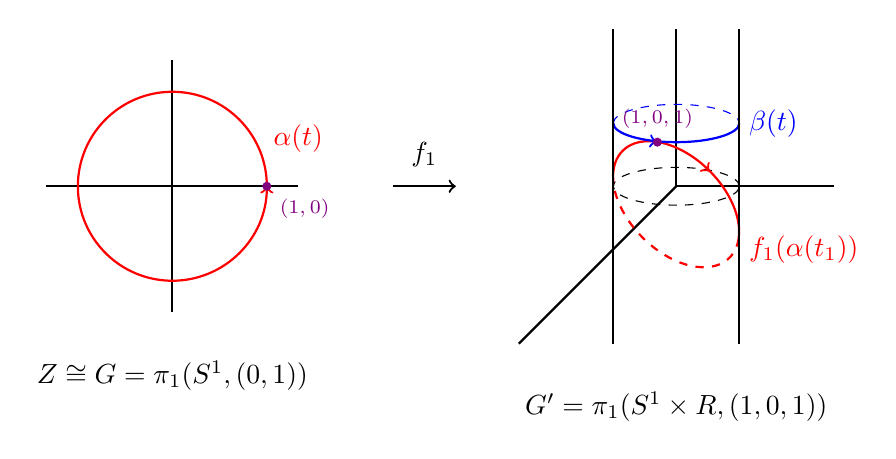
\begin{tikzpicture}[scale=0.8]
            \shorthandoff{>}

            \begin{scope}[shift={(-4,0)}]
                % Ejes
                \draw[thick] (-2,0) -- (2,0);
                \draw[thick] (0,-2) -- (0,2);

                % Circunferencia
                \draw[thick, red, ->] (1.5,0) arc (0:360:1.5 and 1.5);
                \node[red] at (2,0.75) {$\alpha(t)$};

                % Punto
                \node[draw, circle, fill=black,, violet, inner sep=1pt, label={[violet]below right:{\scriptsize $(1,0)$}}] at (1.5,0) {};


                % Leyenda
                \node at (0,-3) {$\bb{Z} \cong G = \pi_1(\bb{S}^1,(0,1))$};

            \end{scope}

            \node at (0,0.5) {$f_1$};
            \draw[thick,->] (-0.5,0) -- (0.5,0);

            \begin{scope}[shift={(4,0)}]
                % Ejes
                \draw[thick] (0,0) -- (0,2.5);
                \draw[thick] (0,0) -- (2.5,0);
                \draw[thick] (0,0) -- (-2.5,-2.5);
                \draw[dashed] (0,0) ellipse (1 and 0.3);

                % f_1(\alpha(t_1))
                \draw[red, thick, dashed, rotate around={-45:(0,-0.3)}] (1.075,0.025)  arc (25:-155:1.2 and 0.75);
                \draw[red, thick, rotate around={-45:(0,-0.3)}] (1.075,0.025)  arc (25:210:1.2 and 0.75);
                \draw[->, red, thick, rotate around={-45:(0,-0.3)}] (0,0.45) ++(-0.02, 0) -- ++(0.01,0);
                \node[red, anchor=west] at (1,-1) {$f_1(\alpha(t_1))$};
                
                % Beta
                \draw[dashed, blue] (-1,1) arc (180:0:1 and 0.3);
                \draw[thick, blue] (-1,1) arc (-180:0:1 and 0.3);
                \draw[->, blue, thick] (-0.3,0.7) ++(-0.02, 0.01) -- ++(0.01,-0.001);
                \node[blue, anchor=west] at (1,1) {$\beta(t)$};

                

                % Punto
                \node[draw, circle, fill=black,, violet, inner sep=1pt, label={[violet]above:{\scriptsize $(1,0,1)$}}] at (-0.3,0.7) {};

                % Cilindro 
                \draw[thick] (-1,-2.5) -- (-1,2.5);
                \draw[thick] (1,-2.5) -- (1,2.5);

                % Leyenda
                \node at (0,-3.5) {$G' = \pi_1(\bb{S}^1 \times \bb{R},(1,0,1))$};
            \end{scope}
        \end{tikzpicture}
    \end{figure}

    podemos ver que $\pi_1(\bb{S}^1,(1,0))$ está generado por $[\alpha]$ donde 
    \begin{gather*}
        \alpha(t) = (\cos(2\pi t), \sen(2\pi t))
    \end{gather*}
    y $\pi_1(\bb{S}^1\times \bb{R}, (1,0,1))$ está generado por $[\beta]$ done 
    \begin{gather*}
        \beta(t) = (\cos(2\pi t), \sen(2\pi t), 1)
    \end{gather*}
    Además es fácil ver en la misma gráfica que
    \begin{gather*}
        f_{1*}([\alpha]) = [f_1 \circ \alpha] = [\beta]\\
        f_{1*}(\pi_1(\bb{S}^1, (1,0))) = \pi_1(\bb{S}^1\times \bb{R}, (1,0,1))
    \end{gather*}
    Ahora calculamos
    \begin{gather*}
        p_*(\pi_1(\bb{S}^1 \times \bb{R}, (1,0,1)))
    \end{gather*}
    Sabemos que 
    \begin{gather*}
        \pi_1(\bb{S}^1 \times \bb{R}, (1,0,1)) = \{[\beta]^n : n\in \bb{Z}\}
    \end{gather*}
    y además
    \begin{align*}
        (p\circ \beta)(t) &= (\cos^2(2\pi t) - \sen^2(2\pi t), 2\cos (2\pi t)\sen(2\pi t), 1) =\\
        &= (\cos(4\pi t), \sen(4\pi t), 1) = (\beta \ast \beta)(t)
    \end{align*}
    por lo que 
    \begin{gather*}
        p_*([\beta]) = [p\circ \beta] = [\beta]^2\\
        p_*(\pi_1(\bb{S}^1 \times \bb{R}, (1,0,1))) = \{[\beta]^{2n} : n\in \bb{Z}\}
    \end{gather*}

    Sabemos por el teorema visto que existe un $\hat{f_1} : \bb{S}^1 \to \bb{S}^1 \times \bb{R}$ levantamiento de $f_1$ con $\hat{f_1}(1,0)=(1,0,1)$ si y solo si se tiene que 
    \begin{gather*}
        f_{1*}(\pi_1(\bb{S}^1, (1,0))) \subseteq p_*(\pi_1(\bb{S}^1 \times \bb{R}, (1,0,1)))
    \end{gather*}
    Como tenemos que 
    \begin{gather*}
        f_{1*}(\pi_1(\bb{S}^1, (1,0))) = \{[\beta]^k : k\in \bb{Z}\} \cong \bb{Z} \\
        p_*(\pi_1(\bb{S}^1 \times \bb{R}, (1,0,1))) = \{[\beta]^{2m}: m\in \bb{Z}\} \cong 2\bb{Z}
    \end{gather*}
    no se dará la inclusión 
    \begin{gather*}
        f_{1*}(\pi_1(\bb{S}^1, (1,0))) \nsubseteq p_*(\pi_1(\bb{S}^1 \times \bb{R}, (1,0,1)))
    \end{gather*}
    y tenemos que no existe $\hat{f_1} : \bb{S}^1 \to \bb{S}^1 \times \bb{R}$ levantamiento de $f_1$ con $\hat{f_1}(1,0)=(1,0,1)$.

    Si tomamos otro punto $r_1$ cualquiera tal que $p(r_1)=(1,0,1)$ ($r_1$ colo podría ser el $(-1,0,1)$) entonces sabemos por un corolario anterior que 
    \begin{gather*}
        p_*(\pi_1(\bb{S}^1\times \bb{R}, r_1)) \text{ es conjugado de } p_*(\pi_1(\bb{S}^1 \times \bb{R}, (1,0,1)))
    \end{gather*}
    Como el grupo total es abeliano, entonces estos dos grupos son idénticos.\\
    
    Veamos qué ocurre con $f_2$. En este caso tenemos que 
    \begin{gather*}
        f_2(1,0) = (1,0,1)
    \end{gather*}
    Además, $[\alpha]$ genera $\pi_1(\bb{S}^1, (1,0))$ y $[\gamma]$ genera $\pi_1(\bb{S}^1 \times \bb{R}, (0,1,1))$ donde 
    \begin{gather*}
        \gamma(t) = \left(\cos\left(2\pi t + \frac{\pi}{2}\right), \sen\left(2\pi t + \frac{\pi}{2}\right), 1\right)
    \end{gather*}
    Queremos calcular $f_2\circ \alpha$:
    \begin{align*}
        (f_2\circ \alpha)(t) &= (-2\cos(2\pi t)\sen(2\pi t), \cos^2(2\pi t) - \sen^2(2\pi t), \cos^2(2\pi t)) = \\
        &= (-\sen(4\pi t), -\cos(4\pi t), \cos^2(2\pi t)) =\\
        &= (\sen(-4\pi t), \cos(-4\pi t), \cos^2(2\pi t)) =\\
        &= \left(\cos\left(\frac{\pi}{2} + 4\pi t\right), \sen\left(\frac{\pi}{2} + 4\pi t\right), \cos^2(2\pi t)\right)
    \end{align*}
    y podemos concluir que 
    \begin{gather*}
        f_{2*}([\alpha]) = [f_2\circ \alpha] = [\gamma \ast \gamma] = [\gamma]^2
    \end{gather*}
    por lo que
    \begin{align*}
        f_{2*}(\pi_1(\bb{S}^1,(1,0))) &= \{[\gamma]^{2n} : n\in \bb{Z}\} =\\
        &= p_*\left(\bb{S}^1 \times \bb{R}, \left(\frac{1}{\sqrt{2}}, \frac{1}{\sqrt{2}}, 1\right), \right) 
    \end{align*}
    y tenemos finalmente que existe el levantamiento $\hat{f_2}$ con $\hat{f_2}(1,0)=(0,1,1)$
\end{ejemplo}